\chapter{Interest Rate Derivatives and Curve Models}
\label{ch:rates_derivatives}
\chaptermark{Interest rate derivatives and curve models}

\Cref{ch:fixed_income_foundations} built the zero curve and priced a
plain-vanilla interest rate swap.  This chapter prices the
\emph{options on} those rates: caps, floors, and swaptions.  The
models that do this (Black'76, Hull--White, BGM/LMM, and SABR)
are the daily tools of a rates Strat.  Understanding how they work,
how they calibrate, and which to reach for in which situation is the
core of what a rates desk does every morning.

\begin{backgroundbox}[Prerequisites]
\begin{itemize}
  \item \Cref{ch:black_scholes}: Black--Scholes, risk-neutral pricing,
    $d_1$/$d_2$, volatility as input.
  \item \Cref{ch:greeks_hedging}: delta, gamma, vega; delta-hedging.
  \item \Cref{ch:fixed_income_foundations}: zero rates $z(T)$,
    discount factors $D(T)$, forward rates $f(T_1,T_2)$, swaps,
    duration.
\end{itemize}
Re-read the relevant chapter if any feel hazy.
\end{backgroundbox}

\subsection*{A concrete scenario before we begin}

A corporate treasurer has issued a \$500~million floating-rate bond
paying 3-month SOFR plus a spread, resetting quarterly for 5~years.
They are happy with today's rates but terrified of a spike.  They want
insurance: if 3-month SOFR exceeds 5\%, someone else pays the
difference.  That contract is a \textbf{cap}, and its price depends on
a model of how rates might move.

A rates trader at Goldman Sachs, asked to quote a 2Y$\times$10Y
receiver swaption struck 50~bps below the forward swap rate, needs:
\begin{enumerate}
  \item The forward swap rate (from the zero curve of
    \cref{ch:fixed_income_foundations}).
  \item The implied volatility at that strike (from the \textbf{SABR
    model} calibrated to the swaption market).
  \item A pricing formula (\textbf{Black'76}) to convert forward,
    strike, and vol into a dollar price.
\end{enumerate}
This chapter teaches each piece.

\begin{historybox}
Interest rate options barely existed before the 1980s.  The cap
market developed in the US in the early 1980s as floating-rate lending
boomed; swaptions followed late in the decade.  Fischer Black's 1976
commodity-futures paper was adapted to rates by mid-1980s
practitioners, and ``Black's model'' became the market standard almost
overnight.  The SABR model (Hagan, Kumar, Lesniewski, Woodward, 2002)
added the smile Black could not capture and remains dominant on rates
desks today \citeHagan.
\end{historybox}


%% ================================================================
\section{Caps, floors, and swaptions}
\label{sec:caps_floors_swaptions}
%% ================================================================

The three most heavily traded rate options (\emph{caps},
\emph{floors}, and \emph{swaptions}) account for most rate-option
volume on dealer desks.  Each is built from a simple block; the trick
is seeing how the pieces fit together.

\subsection{Caplets and caps}

Recall from \cref{ch:fixed_income_foundations} that a floating-rate
borrower pays a reference rate (e.g.\ SOFR) that resets each period.
A \textbf{caplet} is a call option on one future fixing: it pays off
if the rate exceeds a pre-agreed \emph{cap rate} (the strike).

\begin{definition}[Caplet]
\index{caplet|textbf}\index{cap!caplet|textbf}
\label{def:caplet}
A \emph{caplet} with strike $\Kstrike$, notional $N$, reset $T_i$,
payment $T_{i+1} = T_i + \tau$ (accrual $\tau$, e.g.\ 0.5~yr for
semi-annual) pays at $T_{i+1}$:
\begin{equation}
  \text{Caplet payoff} \;=\; N \,\tau \,\max\!\bigl(L(T_i, T_i, T_{i+1}) - \Kstrike,\; 0\bigr),
  \label{eq:caplet_payoff}
\end{equation}
where $L(T_i, T_i, T_{i+1})$ is the floating rate fixed at $T_i$
for $[T_i, T_{i+1}]$.
\end{definition}

$\tau$ converts an annual rate into a dollar amount over the accrual
period; the $\max$ makes it an option.

\begin{definition}[Cap]
\index{cap (rate option)|textbf}
\label{def:cap}
A \emph{cap} is a strip of caplets, one per reset date; it is
literally a portfolio of independent call options on the floating rate.  A
3-year cap on 6-month SOFR with semi-annual resets contains 6~caplets
(months 0, 6, 12, 18, 24, 30), each paying at the end of its accrual
period; a 5-year quarterly-reset cap would contain 20~caplets.
\end{definition}

\begin{intuitionbox}
A cap is insurance for a floating-rate borrower: pay a premium
upfront; if rates rise above $\Kstrike$, the cap pays the difference,
capping your effective borrowing rate at $\Kstrike$.
\end{intuitionbox}

\subsection{Floorlets and floors}

A \textbf{floorlet} is the mirror image: a put option on a single
floating-rate fixing.

\begin{definition}[Floorlet and floor]
\index{floor (rate option)|textbf}\index{floorlet|textbf}
\label{def:floorlet}
A \emph{floorlet} with strike $\Kstrike$ has payoff at $T_{i+1}$:
\begin{equation}
  \text{Floorlet payoff} \;=\; N\,\tau\,\max\!\bigl(\Kstrike - L(T_i, T_i, T_{i+1}),\; 0\bigr).
  \label{eq:floorlet_payoff}
\end{equation}
A \emph{floor} is a strip of floorlets, one per reset date.
\end{definition}

A floor protects a floating-rate \emph{lender} against rates falling
below $\Kstrike$.

\paragraph{Cap--floor parity.}
Long cap and short floor at the same strike replicate a
floating-for-fixed swap:
\begin{equation}
  \text{Cap}(\Kstrike) - \text{Floor}(\Kstrike) = \text{Swap (pay fixed } \Kstrike\text{)}.
  \label{eq:cap_floor_parity}
\end{equation}
The rates analogue of put--call parity (\cref{ch:options_payoffs}).
At the par swap rate $\Kstrike = s_{\text{par}}$, cap and floor have
equal value (swap worth zero at inception).

\begin{keyfactbox}[Cap--floor parity]
\[
  \text{Cap}(K) - \text{Floor}(K) = \text{Payer swap}(K).
\]
When $K$ equals the par swap rate, cap and floor values are equal.
This is the interest-rate analogue of put--call parity.
\end{keyfactbox}

\subsection{Swaptions}

A \textbf{swap} exchanges a floating rate (e.g.\ SOFR) for a fixed
rate: a company with floating-rate debt swaps to fixed to make its
interest costs predictable, and the dealer on the other side earns
the bid--offer.  A \textbf{swaption} is the option, not the
obligation, to enter such a swap at a pre-agreed fixed rate on a
future date, letting a borrower lock in worst-case funding costs
today while walking away if rates move in their favour.

\begin{definition}[Swaption]
\index{swaption|textbf}
\label{def:swaption}
A \emph{swaption} gives the right (not obligation) to enter a swap
at a pre-agreed fixed rate (strike) on a future date (expiry).
\begin{itemize}
  \item \textbf{Payer swaption}: right to pay fixed / receive
    floating.  Profits when rates rise.
  \item \textbf{Receiver swaption}: right to receive fixed / pay
    floating.  Profits when rates fall.
\end{itemize}
\end{definition}

A swaption has two time dimensions: the \textbf{expiry} (when you
decide to exercise) and the \textbf{tenor} (length of the underlying
swap).  Standard notation is ``expiry $\times$ tenor'': a
\textbf{1Y$\times$5Y payer swaption} gives the right, one year from
now, to enter a 5-year payer swap.

\paragraph{Swaption payoff.}
At expiry $T_0$, a payer-swaption holder exercises if the par swap
rate $s(T_0)$ exceeds $\Kstrike$.  The exercise value is the PV of
the annuity stream $(s(T_0) - \Kstrike)$:
\begin{equation}
  \text{Payer swaption payoff at } T_0 \;=\;
    N \,\max\!\bigl(s(T_0) - \Kstrike,\;0\bigr)\,A(T_0),
  \label{eq:swaption_payoff}
\end{equation}
where $A(T_0) = \sum_{i=1}^{n} \tau_i\, D(T_0, T_i)$ is the
\textbf{annuity factor} (present value of a basis point on the swap).

\begin{pitfallbox}[Caps vs.\ swaptions]
Caps and swaptions are \emph{not} interchangeable.  A cap is a basket
of independent options on individual forward rates (one caplet per
period).  A swaption is a single option on a \emph{swap rate}, a
weighted average of forwards.  Forward-rate correlation matters
enormously for swaptions, not for caps.
\end{pitfallbox}


%% ================================================================
\section{Black'76 caplet pricing}
\label{sec:black76}
%% ================================================================

Black--Scholes (\cref{ch:black_scholes}) models spot as GBM.  The
rates analogue is \textbf{Black'76}, developed by Fischer Black for
commodity futures \citeBlackSF.  The idea is simple: model the
\emph{forward rate} as the underlying and reuse the Black--Scholes
formula.

\subsection{Setup: forward rate as underlying}

Under the $T_{i+1}$-forward measure $\Qm^{T_{i+1}}$, the forward rate
$F(t; T_i, T_{i+1})$ is a martingale (a standard result of
arbitrage-free pricing; stated without proof).  Black's model assumes
it follows GBM under this measure:
\begin{equation}
  dF \;=\; \volat_{\text{Black}}\, F\, dW^{T_{i+1}},
  \label{eq:black76_sde}
\end{equation}
where $\volat_{\text{Black}}$ is constant and $W^{T_{i+1}}$ is a
Brownian motion under the forward measure.  There is no drift: the
forward is already a martingale, so its expectation equals today's
forward $F(0; T_i, T_{i+1})$.  Because \cref{eq:black76_sde} has the
same form as Black--Scholes GBM, the pricing formula follows
immediately.

\subsection{The Black'76 caplet formula}

\begin{keyfactbox}[Black'76 caplet formula]
The price at time~0 of a caplet with strike $\Kstrike$, notional $N$,
forward rate $F$, accrual period $\tau$, option expiry $T$, and
Black volatility $\volat$ is:
\begin{equation}
  V_{\text{caplet}} \;=\; D(T+\tau)\;\tau\;N\;\bigl[F\,\CDFN(d_1) - \Kstrike\,\CDFN(d_2)\bigr],
  \label{eq:black76_caplet}
\end{equation}
where
\begin{equation}
  d_1 = \frac{\ln(F/\Kstrike) + \tfrac{1}{2}\volat^2 T}{\volat\sqrt{T}},
  \qquad
  d_2 = d_1 - \volat\sqrt{T},
  \label{eq:black76_d1d2}
\end{equation}
$\CDFN(\cdot)$ is the standard normal CDF, and $D(T+\tau)$ is the
discount factor from today to the payment date $T+\tau$.
\end{keyfactbox}

Same structure as the Black--Scholes call (\cref{ch:black_scholes}):
the forward rate $F$ replaces the forward stock price $Se^{rT}$, and
discounting is to the \emph{payment date} $T+\tau$, not the option
expiry $T$.

\paragraph{Floorlet formula.}
By cap--floor parity:
\begin{equation}
  V_{\text{floorlet}} \;=\; D(T+\tau)\;\tau\;N\;\bigl[\Kstrike\,\CDFN(-d_2) - F\,\CDFN(-d_1)\bigr].
  \label{eq:black76_floorlet}
\end{equation}

\paragraph{Swaption formula.}
Black also prices swaptions.  A payer swaption with strike $\Kstrike$,
annuity $A$, and forward swap rate $s$:
\begin{equation}
  V_{\text{payer}} \;=\; N\;A\;\bigl[s\,\CDFN(d_1) - \Kstrike\,\CDFN(d_2)\bigr],
  \label{eq:black_swaption}
\end{equation}
with $d_1, d_2$ from \cref{eq:black76_d1d2} using swaption vol
$\volat_{\text{swap}}$ and $s$ in place of $F$.

\subsection{Worked example: pricing a caplet}
\label{sec:caplet_worked}

Parameters:
\begin{center}
\begin{tabular}{ll}
  \toprule
  Parameter & Value \\
  \midrule
  Notional $N$ & \$1{,}000{,}000 \\
  Strike $\Kstrike$ & 4.0\% \\
  Forward SOFR rate $F$ & 4.5\% \\
  Black volatility $\volat$ & 20\% \\
  Option expiry $T$ & 1.0 year \\
  Accrual period $\tau$ & 0.5 years \\
  Continuously compounded zero rate & 4.3\% (flat) \\
  \bottomrule
\end{tabular}
\end{center}

\paragraph{Step 1: Discount factor.}
Pays at $T + \tau = 1.5$~yr: $D(1.5) = e^{-0.043 \times 1.5} = 0.93754$.

\paragraph{Step 2: $d_1, d_2$.}
\[
  d_1 = \frac{\ln(1.125) + 0.02}{0.20}
      = \frac{0.13778}{0.20} = 0.6889,
  \qquad
  d_2 = 0.6889 - 0.20 = 0.4889.
\]

\paragraph{Step 3: Normal CDFs.}
$\CDFN(0.6889) = 0.7546$, $\CDFN(0.4889) = 0.6875$.

\paragraph{Step 4: Apply the formula.}
\begin{align}
  V_{\text{caplet}} &= D(1.5) \;\tau\; N \;\bigl[F\,\CDFN(d_1) - \Kstrike\,\CDFN(d_2)\bigr] \notag \\
    &= 0.93754 \times 0.5 \times 1{,}000{,}000 \times
       \bigl[0.045 \times 0.7546 - 0.04 \times 0.6875\bigr] \notag \\
    &= 0.93754 \times 0.5 \times 1{,}000{,}000 \times
       \bigl[0.033957 - 0.027500\bigr] \notag \\
    &= 0.93754 \times 0.5 \times 1{,}000{,}000 \times 0.006457 \notag \\
    &= \$3{,}025.
    \label{eq:caplet_worked_result}
\end{align}

The caplet is worth about \textbf{\$3{,}025} ($\approx 30.25$~bps of
notional): the upfront premium for protection against 6-month SOFR
exceeding 4\% at the 1-year reset.

\begin{intuitionbox}
The caplet is forward ITM (4.5\% $>$ 4.0\% strike), hence $\CDFN(d_1),
\CDFN(d_2) > 0.5$.  The dollar value is modest because the option
pays on a single 6-month period of the notional, not the full
notional as in an equity option.
\end{intuitionbox}

\subsection{Python implementation}

\begin{lstlisting}[caption={Black'76 caplet pricer},label={lst:black76_caplet}]
import math
from scipy.stats import norm

def black76_caplet(F, K, sigma, T, tau, D_pay, N=1e6):
    """Black'76 caplet: F=forward, K=strike, sigma=Black vol,
    T=expiry (yr), tau=accrual (yr), D_pay=DF to T+tau, N=notional."""
    d1 = (math.log(F / K) + 0.5 * sigma**2 * T) / (sigma * math.sqrt(T))
    d2 = d1 - sigma * math.sqrt(T)
    return D_pay * tau * N * (F * norm.cdf(d1) - K * norm.cdf(d2))

# Worked example
D = math.exp(-0.043 * 1.5)           # 0.93754
price = black76_caplet(0.045, 0.04, 0.20, 1.0, 0.5, D)
print(f"Caplet = ${price:,.2f}")      # $3,025.11
\end{lstlisting}


%% ================================================================
\section{Hull--White short-rate model (outline)}
\label{sec:hull_white}
%% ================================================================

Black prices each caplet or swaption independently with its own vol
and cannot enforce consistency across instruments: the vol fitting a
1Y caplet need not match the vol fitting a 1Y$\times$5Y swaption.
For exotics (Bermudan swaptions, callable bonds, range accruals) we
need a model of the entire term structure, evolving all rates
simultaneously.

The \textbf{Hull--White model} \citeHW\ is the workhorse one-factor
short-rate model.  It extends Vasicek/Ornstein--Uhlenbeck with a
time-dependent drift that fits today's zero curve exactly.

\subsection{The model}

\begin{keyfactbox}[Hull--White model]
The short rate $r_t$ follows:
\begin{equation}
  dr_t = \bigl[\theta(t) - a\, r_t\bigr]\,dt + \volat\, dW_t,
  \label{eq:hull_white}
\end{equation}
where:
\begin{itemize}
  \item $a > 0$ is the \textbf{mean-reversion speed}: the rate is
    pulled back towards a time-dependent level $\theta(t)/a$.
  \item $\volat > 0$ is the \textbf{short-rate volatility}: the
    instantaneous standard deviation of rate changes.
  \item $\theta(t)$ is a \textbf{deterministic function of time},
    chosen so that the model exactly reproduces today's zero curve.
\end{itemize}
\end{keyfactbox}

\paragraph{Why $\theta(t)$ matters.}
Plain Vasicek has constant $\theta$, so its implied zero curve is
determined by $(a, \theta)$ alone and generally will not match the
market.  Hull--White replaces constant $\theta$ with $\theta(t)$
calibrated to fit the market curve exactly \citeHull:
\begin{equation}
  \theta(t) \;=\; \frac{\partial f^M(0,t)}{\partial t} + a\,f^M(0,t)
    + \frac{\volat^2}{2a}\bigl(1 - e^{-2at}\bigr),
  \label{eq:hw_theta_calib}
\end{equation}
where $f^M(0,t)$ is the market instantaneous forward at maturity $t$.

\paragraph{Bond pricing.}
Under Hull--White, a zero-coupon bond has closed-form price:
\begin{equation}
  P(t,T) = A(t,T)\,\exp\!\bigl[-B(t,T)\,r_t\bigr],
  \label{eq:hw_bond}
\end{equation}
where $B(t,T) = \frac{1}{a}\bigl(1 - e^{-a(T-t)}\bigr)$ and $A(t,T)$
is set by the initial term structure (see \citeHull, Ch~31).  This
tractability is the model's strength: bonds, caps, and European
swaptions all have closed-form prices.

\paragraph{Swaption pricing.}
A European swaption is an option on the fixed-leg coupon bond.
Jamshidian's trick reduces it to a portfolio of zero-coupon bond
options, each with a closed-form Hull--White price (details in
\citeHull, Ch~31).  The practical fact:

\begin{keyfactbox}[Hull--White for European swaptions]
European swaptions have a closed-form Hull--White price.  Free
parameters $(a, \volat)$ are calibrated to market swaptions.  With
only two parameters, the model fits a limited slice of the swaption
matrix, typically one row or column.
\end{keyfactbox}

\subsection{Strengths and limitations}

\begin{center}
\begin{tabular}{p{0.43\textwidth}p{0.43\textwidth}}
  \toprule
  \textbf{Strengths} & \textbf{Limitations} \\
  \midrule
  Exact fit to today's zero curve &
    One factor: all rates move in parallel \\[3pt]
  Closed-form bond and swaption prices &
    Cannot fit the full swaption matrix \\[3pt]
  Mean reversion prevents rates drifting to unreasonable levels &
    Normal model: rates can go negative (a feature post-2010, a bug
    before) \\[3pt]
  Fast calibration (2 parameters) &
    No smile / skew \\
  \bottomrule
\end{tabular}
\end{center}

The lack of smile is Hull--White's main limitation.  It prices
European options with a single vol per strike, which is fine for ATM
risk but inadequate for away-from-ATM instruments.  Smile-consistent
pricing needs SABR (\cref{sec:sabr}).

\subsection{Numerical implementation: the trinomial tree}

For Bermudan swaptions and other early-exercise products, Hull--White
is implemented on a \textbf{trinomial tree}: at each step $\Delta t$
the rate can move up, flat, or down, with:
\begin{itemize}
  \item branch spacing $\Delta r = \volat\sqrt{3\Delta t}$;
  \item probabilities chosen to match the model's mean and variance;
  \item $\theta(t)$ embedded by placing the central node at the
    mean-reverting level.
\end{itemize}
Pricing is backward induction from terminal nodes (the rates analogue
of the equity binomial tree, \cref{ch:black_scholes}, with three
branches).  At each Bermudan exercise date, take the max of
continuation and exercise value.  This is how Bermudan swaptions are
priced in practice.

\begin{intuitionbox}
The Hull--White trinomial tree is the rates analogue of
Cox--Ross--Rubinstein.  Key difference: it is calibrated to the
entire initial term structure, not just one spot and vol: $\theta(t)$
bends the tree so today's bond prices are recovered exactly.
\end{intuitionbox}


%% ================================================================
\section{The BGM / Libor Market Model (LMM) as a concept}
\label{sec:bgm}
%% ================================================================

Hull--White works with the abstract short rate $r_t$, but traders
observe and quote \emph{discrete-tenor forward rates} (3M SOFR, 6M
SOFR, \ldots).  The \textbf{Brace--G\k{a}tarek--Musiela (BGM) model},
a.k.a.\ the \textbf{Libor Market Model (LMM)}, models these
observable forwards directly \citeBGM.

\subsection{The SDE}

The model specifies forward rates $\{F_k(t)\}$ for $k=1,\ldots,n$,
where $F_k(t)$ is the time-$t$ forward for period $[T_k, T_{k+1}]$.
Under the $T_{k+1}$-forward measure:
\begin{equation}
  dF_k(t) \;=\; \volat_k(t)\, F_k(t)\, dW_k^{T_{k+1}}(t),
  \label{eq:bgm_sde}
\end{equation}
where $\volat_k(t)$ is a deterministic vol function.  Under any other
measure, drift terms depending on forward-rate correlations appear
(derived in \citeHull, Ch~32).

\paragraph{Key property: caplets are Black-priced by construction.}
Each $F_k$ is log-normal under its own forward measure, so every
caplet is priced exactly by Black'76 with vol $\volat_k(T_k)$, read
directly from market cap quotes.  BGM is built to reproduce the cap
market automatically.

\subsection{What about swaptions?}

Swaptions are harder.  A swap rate is a weighted average of forwards:
\begin{equation}
  s(t) = \frac{\sum_{k} \tau_k\, D(t, T_{k+1})\, F_k(t)}
              {\sum_{k} \tau_k\, D(t, T_{k+1})}.
\end{equation}
Even with each $F_k$ log-normal, $s(t)$ is not (ratio of sums of
log-normals).  Swaption prices in BGM have no closed form.  Two
practical approaches:
\begin{enumerate}
  \item \textbf{Monte Carlo}: simulate joint forward evolution,
    compute swap rate at expiry, average the discounted payoff.
    Accurate but slow; used for exotics.
  \item \textbf{Analytical approximations}: freeze the weights at
    $t=0$, yielding an approximately log-normal swap rate and a
    Black-like swaption formula, accurate enough for many purposes
    \citeHull.
\end{enumerate}

\begin{keyfactbox}[BGM / LMM: key facts]
\begin{itemize}
  \item Models observable forwards directly, not the short rate.
  \item Caplets are Black-priced by construction, so it fits the cap
    market automatically.
  \item Swaptions need MC or analytical approximations.
  \item Requires a forward-rate \textbf{correlation matrix} (the main
    calibration challenge).
  \item Industry standard for exotics (Bermudans, CMS, range accruals).
\end{itemize}
\end{keyfactbox}

\begin{pitfallbox}[BGM does not mean ``log-normal swaptions'']
BGM does \emph{not} imply log-normal swap rates.  The forwards are
log-normal; the swap rate (a weighted average) is not.  Pricing
swaptions as if the swap rate were log-normal is a convenient
approximation, not an exact result.
\end{pitfallbox}


%% ================================================================
\section{SABR: stochastic volatility for rates}
\label{sec:sabr}
%% ================================================================

Black assumes constant vol per forward, but the market quotes
strike-dependent implied vols, the smile/skew seen for equities in
\cref{ch:vol_surface}.  The \textbf{SABR model} (Stochastic Alpha
Beta Rho) is the rates-desk standard for capturing this \citeHagan.

SABR does not replace Black'76 or BGM.  It is a volatility model
producing a Black-vol smile across strikes; those vols then feed
Black's formula for prices.

\subsection{The SABR SDEs}

Two coupled SDEs for the forward $F_t$ and its instantaneous vol
$\alpha_t$:

\begin{keyfactbox}[SABR model]
\begin{align}
  dF_t &= \alpha_t\, F_t^{\beta}\, dW_1(t), \label{eq:sabr_F} \\
  d\alpha_t &= \nu\, \alpha_t\, dW_2(t), \label{eq:sabr_alpha}
\end{align}
with $F_0 = F$, $\alpha_0 = \alpha$, and correlated Brownians
$dW_1\,dW_2 = \rho\,dt$, $\rho \in [-1,1]$.  Four parameters:
\begin{itemize}
  \item $\alpha > 0$: initial vol level.
  \item $\beta \in [0,1]$: backbone / CEV exponent.
  \item $\rho \in (-1,1)$: rate-vol correlation.
  \item $\nu > 0$: vol-of-vol.
\end{itemize}
\end{keyfactbox}

\paragraph{Special cases.}
$\beta=1, \nu=0$: log-normal (Black).  $\beta=0, \nu=0$: normal
(Bachelier).  $\beta=0.5$: square-root CEV backbone, common for rates.

\subsection{Hagan's approximation formula}

Hagan et al.\ derived a closed-form approximation for the Black
implied vol as a function of strike \citeHagan; no numerical SDE
solving is needed.  For $F \neq K$:
\begin{equation}
  \volat_{\text{Black}}(K) \;=\;
    \frac{\alpha}{(FK)^{(1-\beta)/2}
      \Bigl[1 + \frac{(1-\beta)^2}{24}\ln^2\!\frac{F}{K}
        + \frac{(1-\beta)^4}{1920}\ln^4\!\frac{F}{K}\Bigr]}
    \;\cdot\;
    \frac{z}{x(z)}
    \;\cdot\;
    \Bigl[1 + \epsilon\, T\Bigr],
  \label{eq:hagan_sabr}
\end{equation}
where
\begin{align}
  z &= \frac{\nu}{\alpha}\,(FK)^{(1-\beta)/2}\,\ln\frac{F}{K},
  \label{eq:hagan_z} \\
  x(z) &= \ln\!\left(\frac{\sqrt{1 - 2\rho z + z^2} + z - \rho}{1 - \rho}\right),
  \label{eq:hagan_xz} \\
  \epsilon &= \frac{(1-\beta)^2}{24}\,\frac{\alpha^2}{(FK)^{1-\beta}}
    + \frac{\rho\beta\nu\alpha}{4\,(FK)^{(1-\beta)/2}}
    + \frac{(2-3\rho^2)\,\nu^2}{24}.
  \label{eq:hagan_epsilon}
\end{align}
At the money ($K = F$), the formula simplifies to:
\begin{equation}
  \volat_{\text{ATM}} \;=\;
    \frac{\alpha}{F^{1-\beta}}\;
    \Bigl[1 + \epsilon_{\text{ATM}}\, T\Bigr],
  \label{eq:hagan_atm}
\end{equation}
with $\epsilon_{\text{ATM}}$ given by \cref{eq:hagan_epsilon} evaluated at
$K = F$.

\begin{intuitionbox}
SABR gives a \textbf{recipe}: plug in $(\alpha, \beta, \rho, \nu)$
and strike $K$, out comes the Black vol.  The four parameters shape
the smile:
\begin{itemize}
  \item $\beta$ = \textbf{backbone}: how ATM vol moves with the
    forward.
  \item $\rho$ = \textbf{skew}: $\rho < 0$ means vol rises as rates
    fall (typical for rates).
  \item $\nu$ = \textbf{wings}: higher $\nu$ $\Rightarrow$ fatter
    tails, richer OTM options.
  \item $\alpha$ = overall \textbf{level} of ATM vol.
\end{itemize}
One-liner: ``$\beta$ = backbone, $\rho$ = skew, $\nu$ = wings.''
\end{intuitionbox}

\subsection{Calibration workflow}
\label{sec:sabr_calib}

Given market implied vols at several strikes for a given expiry/tenor,
find $(\alpha, \beta, \rho, \nu)$ that best reproduce them.

\paragraph{Step 1: Fix $\beta$.}
$\beta$ is almost always fixed: $\beta=0.5$ (most popular for rates,
square-root backbone), $\beta=0$ (normal SABR, for negative-rate
environments), $\beta=1$ (log-normal, for equities/commodities).
Three parameters remain: $\alpha, \rho, \nu$.

\paragraph{Step 2: Fit $\alpha$ from ATM vol.}
Given $\volat_{\text{ATM}}^{\text{mkt}}$ and $(\beta, \rho, \nu)$,
invert \cref{eq:hagan_atm} for $\alpha$.  Inner loop: for each trial
$(\rho, \nu)$, solve for $\alpha$, then evaluate the smile.

\paragraph{Step 3: Minimise smile error.}
Search $(\rho, \nu)$ to minimise squared error vs.\ market vols across
quoted strikes:
\begin{equation}
  \min_{\rho, \nu}\;\sum_{j=1}^{m}
    \bigl[\volat_{\text{SABR}}(K_j; \alpha(\rho,\nu), \beta, \rho, \nu)
      - \volat_{\text{mkt}}(K_j)\bigr]^2.
  \label{eq:sabr_calib_obj}
\end{equation}
This is a 2D optimisation, fast enough to run in milliseconds, which
is critical because rates desks recalibrate SABR at every (expiry,
tenor) cell of the swaption matrix every morning.

\subsection{Worked example: qualitative SABR smile}
\label{sec:sabr_worked}

Consider a 1Y$\times$5Y swaption with $F = 4.0\%$, $T = 1$~year.  Fix
$\beta = 0.5$; calibration yields $\alpha = 0.02$, $\rho = -0.30$,
$\nu = 0.40$.  Hagan's formula at five strikes:

\begin{center}
\begin{tabular}{cccc}
  \toprule
  Strike & Moneyness & SABR IV (\%) & Shape role \\
  \midrule
  2.00\% & $-200$ bps & 19.5 & Left wing ($\nu$) + skew ($\rho < 0$) \\
  3.00\% & $-100$ bps & 13.7 & Skew \\
  4.00\% & ATM        & 10.1 & Level ($\alpha$) \\
  5.00\% & $+100$ bps &  9.6 & Slight downtick from skew \\
  6.00\% & $+200$ bps & 10.6 & Right wing ($\nu$) \\
  \bottomrule
\end{tabular}
\end{center}

Clear \emph{negative skew}: vol is higher for low strikes (rates
falling) than high (rates rising), driven by $\rho = -0.30$: when
the forward drops, $\alpha_t$ rises, pushing vol higher.  Wings are
elevated by $\nu = 0.40$: higher vol-of-vol $\Rightarrow$ fatter
tails $\Rightarrow$ richer OTM options.

\begin{center}
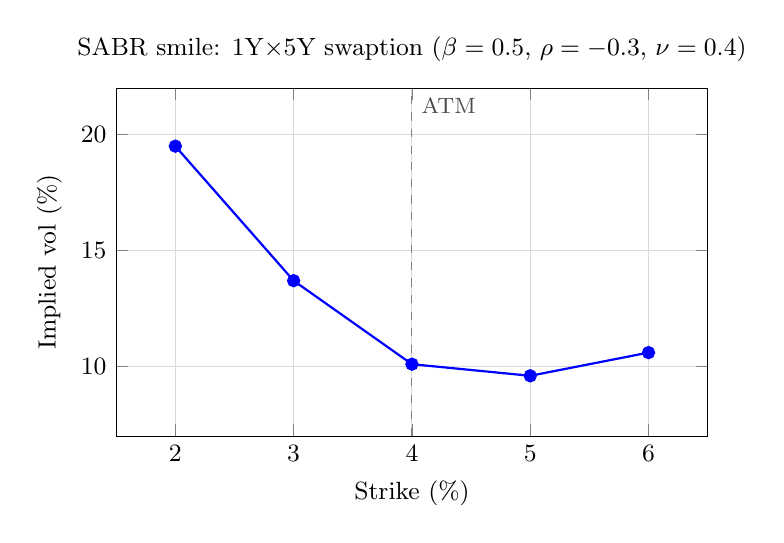
\begin{tikzpicture}
  \begin{axis}[
    width=0.75\textwidth,
    height=6cm,
    xlabel={Strike (\%)},
    ylabel={Implied vol (\%)},
    title={SABR smile: 1Y$\times$5Y swaption ($\beta=0.5$, $\rho=-0.3$, $\nu=0.4$)},
    xmin=1.5, xmax=6.5,
    ymin=7, ymax=22,
    grid=major,
    grid style={gray!30},
    mark options={solid},
    title style={font=\small},
    label style={font=\small},
    tick label style={font=\small},
  ]
  \addplot[blue, thick, mark=*] coordinates {
    (2.0, 19.5)
    (3.0, 13.7)
    (4.0, 10.1)
    (5.0,  9.6)
    (6.0, 10.6)
  };
  \draw[dashed, gray] (axis cs:4.0,7) -- (axis cs:4.0,22)
    node[below right, font=\footnotesize, text=black!70] {ATM};
  \end{axis}
\end{tikzpicture}
\end{center}

The negative skew is visible; the right wing is slightly elevated
from $\nu$.

\paragraph{Effect of changing $\rho$.}
Flipping $\rho$ from $-0.30$ to $+0.30$ reverses the skew: vol higher
at high strikes, lower at low.  In rates, $\rho$ is almost always
negative (flight-to-quality: rates fall, vol spikes); in some
commodities it is positive.

\paragraph{Effect of changing $\nu$.}
Raising $\nu$ from 0.4 to 0.8 lifts both wings dramatically while
leaving ATM nearly unchanged: higher vol-of-vol fattens the tails.
$\nu = 0$ collapses the smile to flat (Black).

\begin{pitfallbox}[SABR is a smile interpolator]
SABR is a snapshot of the smile: it does not describe how the
smile evolves over time (its dynamics are known to be unrealistic;
the backbone moves too predictably).  Many desks overlay SABR with
empirical adjustments for hedging.  Use SABR for \emph{marking}
(consistent vols across strikes), not for predicting smile moves.
\end{pitfallbox}

\subsection{SABR parameter intuition}

\begin{keyfactbox}[SABR parameters --- summary]
\begin{center}
\begin{tabular}{clp{0.55\textwidth}}
  \toprule
  Parameter & Name & Interpretation \\
  \midrule
  $\alpha$ & Level & Overall ATM vol level. \\
  $\beta$ & Backbone &
    How ATM vol moves with the forward.  $\beta=1$: \% vol constant;
    $\beta=0$: bp vol constant. \\
  $\rho$ & Skew &
    Rate-vol correlation.  $\rho<0$ (typical): vol rises as rates fall
    $\Rightarrow$ downward skew. \\
  $\nu$ & Vol-of-vol &
    Curvature (wings).  Higher $\nu$ $\Rightarrow$ fatter
    tails $\Rightarrow$ more expensive out-of-the-money options. \\
  \bottomrule
\end{tabular}
\end{center}
\end{keyfactbox}


%% ================================================================
\section{Connecting the models}
\label{sec:models_comparison}
%% ================================================================

The four models serve different purposes:

\begin{center}
\begin{tabular}{p{0.16\textwidth}p{0.22\textwidth}p{0.22\textwidth}p{0.22\textwidth}}
  \toprule
  \textbf{Model} & \textbf{What it models} & \textbf{Primary use} & \textbf{Limitation} \\
  \midrule
  Black'76 &
    Single forward rate (log-normal) &
    Vanilla caps/floors, European swaptions &
    Flat smile per instrument \\[3pt]
  Hull--White &
    Short rate (normal, mean-reverting) &
    Bermudan swaptions, callable bonds &
    One factor, no smile \\[3pt]
  BGM/LMM &
    All forward rates jointly &
    Exotic rate products, path-dependent payoffs &
    Needs correlation matrix, MC simulation \\[3pt]
  SABR &
    Smile/skew for a single forward &
    Strike interpolation, vol cube &
    Static snapshot, not dynamics \\
  \bottomrule
\end{tabular}
\end{center}

A rates desk uses all four in concert:
\begin{enumerate}
  \item \textbf{SABR} generates the implied-vol smile at each
    expiry/tenor grid point.
  \item \textbf{Black'76} converts those implied vols into prices for
    vanilla caps, floors, and European swaptions.
  \item \textbf{Hull--White} or \textbf{BGM/LMM} prices exotics
    (Bermudans, CMS caps, callable bonds) using the SABR-calibrated
    smile as input.
\end{enumerate}

\subsection{The swaption matrix and vol cube}

The \textbf{swaption matrix} is a 2D grid with expiries as rows and
swap tenors as columns; each cell holds the ATM Black vol for that
(expiry, tenor) pair.  Typical shape:

\begin{center}
\begin{tabular}{l ccccc}
  \toprule
  & \multicolumn{5}{c}{\textbf{Swap tenor}} \\
  \cmidrule(lr){2-6}
  \textbf{Expiry} & 1Y & 2Y & 5Y & 10Y & 30Y \\
  \midrule
  1M  & 45.2 & 38.1 & 24.5 & 18.3 & 14.1 \\
  3M  & 42.8 & 36.5 & 23.8 & 17.9 & 13.8 \\
  6M  & 39.1 & 34.2 & 22.9 & 17.2 & 13.5 \\
  1Y  & 35.6 & 31.5 & 21.4 & 16.5 & 13.1 \\
  2Y  & 30.2 & 27.8 & 19.8 & 15.6 & 12.7 \\
  5Y  & 24.1 & 22.5 & 17.3 & 14.2 & 12.0 \\
  10Y & 19.8 & 18.9 & 15.1 & 13.0 & 11.3 \\
  \bottomrule
\end{tabular}
\end{center}

\noindent (Values in \% Black vol.  These are illustrative.)

Pattern: vols are highest top-left (short expiries on short-tenor
swaps) and lowest bottom-right.  Short-dated options have high
\% vol because rates can move sharply over a short horizon relative to
their level; long-tenor swap rates are averages of many forwards and
are smoother.

The \textbf{vol cube} extends this to 3D by adding a strike axis.  At
each (expiry, tenor) cell, replace the single ATM vol with a
SABR-calibrated smile, a function from strike to implied vol:
\[
  (\text{expiry}, \;\text{tenor}, \;\text{strike}) \;\longmapsto\; \volat_{\text{Black}}.
\]
This 3D object is the rates desk's central data structure.  Every
vanilla price, exotic calibration, and risk report begins with a
query to the vol cube.


%% ================================================================
\section{Prosperity and industry connections}
\label{sec:rates_deriv_connections}
%% ================================================================

\begin{prosperitybox}
The SABR workflow (observe prices, extract implied vols, fit a
parametric smile, re-price) mirrors the vol-surface calibration of
\cref{ch:vol_surface}.  In Prosperity's Volcanic Rock Vouchers you
did exactly this: observe bot option prices, back out vols, fit,
quote.  The rates version applies the same logic to caps and
swaptions.
\end{prosperitybox}

\begin{gsbox}
On a GS rates desk, the Strat owns the \textbf{SABR calibration
pipeline}.  Daily workflow:
\begin{enumerate}
  \item \textbf{Pre-open:} pull overnight broker quotes and
    exchange-traded cap/swaption prices (Black vols at standard
    strikes).
  \item \textbf{Calibration:} at each (expiry, tenor) cell, fit
    $(\alpha, \rho, \nu)$ with $\beta$ fixed.  Result: the
    \textbf{vol cube} (expiry $\times$ tenor $\times$ strike).
  \item \textbf{Pricing:} the cube feeds the pricing engine (SecDB at
    GS).  Traders price any rate option by interpolating the SABR
    surface.
  \item \textbf{Risk:} Greeks (delta, vega, gamma) via bumping the
    surface; vega is reported per expiry/tenor bucket.  The Strat
    watches for calibration breaks (sudden jumps in $\rho$ or $\nu$
    from bad input data).
\end{enumerate}
``The Strat runs the vol cube'' means exactly this.
\end{gsbox}


%% ================================================================
\section*{Key facts to memorise}
\label{sec:rates_deriv_keyfacts}
%% ================================================================

\begin{keyfactbox}[Chapter summary --- interest rate derivatives]
\begin{enumerate}
  \item \textbf{Cap} = strip of caplets (calls on forwards);
    \textbf{floor} = strip of floorlets (puts).  Cap $-$ Floor = payer
    swap at the same strike.
  \item A \textbf{swaption} is an option to enter a swap.  Payer =
    call on swap rate; receiver = put.
  \item \textbf{Black'76} prices caplets/swaptions by treating the
    forward (swap) rate as a log-normal martingale under the forward
    measure.  Same structure as Black--Scholes.
  \item \textbf{Hull--White}: $dr = [\theta(t) - ar]\,dt + \sigma\,dW$,
    with $\theta(t)$ fitting today's zero curve exactly.  Closed-form
    bonds and swaptions; no smile.
  \item \textbf{BGM/LMM} models forwards directly as log-normal.
    Caplets are Black-priced by construction; swaptions need MC or
    approximations.  Industry standard for exotics.
  \item \textbf{SABR} ($dF = \alpha F^\beta dW_1$, $d\alpha = \nu
    \alpha\,dW_2$, $\rho = \text{Corr}$) is the standard smile model;
    Hagan's formula gives closed-form implied vol vs.\ strike.
  \item SABR parameters: $\alpha$ = level, $\beta$ = backbone, $\rho$
    = skew, $\nu$ = wings.  Fix $\beta$, fit the rest.
  \item The \textbf{vol cube} (expiry $\times$ tenor $\times$ strike)
    comes from SABR at each grid point; it is the central rates-desk
    object.
  \item Flow: SABR $\to$ smile $\to$ Black'76 prices $\to$ Hull--White
    / BGM for exotics.
  \item Rates Strats own the pipeline: quotes in, vol cube out,
    pricing and risk downstream.
\end{enumerate}
\end{keyfactbox}
